\documentclass[11pt, answers]{exam}
\usepackage[utf8]{inputenc}
\usepackage[T1]{fontenc}
\usepackage{amsmath, amssymb, amsopn, color, tikz, mathtools}
\usepackage[margin=1in]{geometry}
\usepackage{titlesec}
\usepackage{tipa}
\usepackage{hyperref}


% Style
\setlength\parindent{0pt}
\shadedsolutions

% Define course info
\def\semester{2019-2020}
\def\course{Modèles Aléatoires Discrets M1}
\def\name{P.-O. Goffard \& Rémy Poudevigne}
%\def\quizdate{10/5, 10/6}
\def\hwknum{}
%\def\title{\MakeUppercase{Homework \hwknum -- quiz \quizdate }}
\def\title{\MakeUppercase{TD 1: Chaine de Markov}}

% Define commands
\def\Bin{\operatorname{Bin}}
\def\Geom{\operatorname{Geom}}
\def\Pois{\operatorname{Pois}}
\def\Exp{\operatorname{Exp}}
\newcommand{\E}{\mathbb E}            % blackboard E
\newcommand{\bP}{\mathbb P}            % blackboard P
\newcommand{\Var}{\text{Var}}            % blackboard P
\newcommand{\Om}{\Omega}            % blackboard P
\newcommand{\om}{\omega}            % blackboard P
\newcommand{\N}{\mathbb N}            % blackboard P
\newcommand{\R}{\mathbb R}            % blackboard P
\newcommand{\A}{\mathcal A}            % blackboard P
\def \si {\sigma}
\def \la {\lambda}
\def \al {\alpha}
% \def\e*{\end{eqnarray*}}
\def \di{\displaystyle}

\def \E{\mathbb E}
\def \N{\mathbb N}
\def \Z{\mathbb Z}
\def \NZ{\mathbb{N}_0}
\def \I{\mathbb I}
\def \w{\widehat}
\def \P {\mathbb P}
\def \V{\mathbb V}


\newcommand{\CL}{\mathbb{C}}
\newcommand{\RL}{\mathbb{R}}
\newcommand{\nat}{{\mathbb N}}
\newcommand{\Laplace}{\mathscr{L}}
\newcommand{\e}{\mathrm{e}}
\newcommand{\ve}{\bm{\mathrm{e}}} % vector e

\renewcommand{\L}{\mathcal{L}} % e.g. L^2 loss.

\newcommand{\ih}{\mathrm{i}}
\newcommand{\oh}{{\mathrm{o}}}
\newcommand{\Oh}{{\mathcal{O}}}


\newcommand{\Norm}{\mathcal{N}}
\newcommand{\LN}{\mathcal{LN}}
\newcommand{\SLN}{\mathcal{SLN}}

\renewcommand{\Pr}{\mathbb{P}}
\newcommand{\Ind}{\mathbb I}
\newcommand\bfsigma{\bm{\sigma}}
\newcommand\bfSigma{\bm{\Sigma}}
\newcommand\bfLambda{\bm{\Lambda}}
\newcommand{\stimes}{{\times}}
\def \limsup{\underset{n\rightarrow+\infty}{\overline{\lim}}}
\def \liminf{\underset{n\rightarrow+\infty}{\underline{\lim}}}
\def\euro{\mbox{\raisebox{.25ex}{{\it =}}\hspace{-.5em}{\sf C}}}
  \everymath{\displaystyle}
% \newcommand{\limsup}{\overline{\lim}\,}            % blackboard P
% \newcommand{\liminf}{\underline{\lim}\,}            % blackboard P

\begin{document}

% Heading
{\center \textsc{\Large\title}\\
	\vspace*{1em}
	\course -- \semester\\
	\name\\
	\vspace*{2em}
	\hrule
\vspace*{2em}}
\begin{questions}
\question Soit $(X_n)_{n\geq0}$ une chaîne de Markov sur $\{1,2,3\}$ de matrice de transition ($p\in[0,1]$):
\[Q=\begin{pmatrix}
0 & 1 & 0 \\
0 & 2/3 & 1/3 \\
p & 1-p & 0
\end{pmatrix}\]
\begin{parts}
\part Dessiner le graphe de cette chaîne de Markov.
\begin{solution}
La chaîne de Markov est donnée par le graphe suivant :
\[
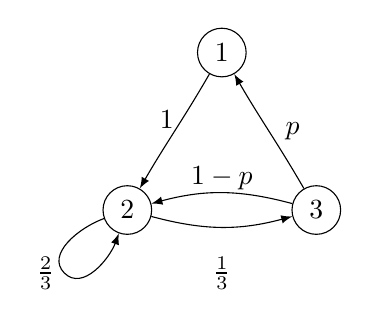
\begin{tikzpicture}
\node[draw,circle] (1)at(0,2){1};
\node[draw,circle] (2)at(-1.2,0){2};
\node[draw,circle] (3)at(1.2,0){3};
\draw[->,>=latex] (1) to[out=240,in=60] (2);
\draw[-,>=latex] (2) to[out=200,in=135] (-2.0,-0.8)node[left]{$\frac{2}{3}$};
\draw[->,>=latex] (-2.0,-0.8)node{} to[out=-45,in=250] (2);
\draw[->,>=latex] (2) to[out=-15,in=195] (3);
\draw[->,>=latex] (3) to[out=120,in=-60] (1);
\draw[->,>=latex] (3) to[out=165,in=15] (2);
\node at(-0.7,1.15) {$1$};
\node at(0,-0.8) {$\frac{1}{3}$};
\node at(0,0.4) {$1-p$};
\node at(0.9,1) {$p$};
\end{tikzpicture}
\]
\end{solution}
\part Calculer $\P (X_1 = 1|X_0 = 1)$, $\P (X_2 = 1|X_0 = 1)$, $\P (X_3 = 1|X_0 = 1)$, $\P (X_4 = 1|X_0 = 1)$, $\P (X_1 = 2|X_0 = 2)$, $\P (X_2 = 2|X_0 = 2)$ et $\P (X_3 = 2|X_0 = 2)$.
\begin{solution}
Pour calculer $\P (X_1 = 1|X_0 = 1)$, $\P (X_2 = 1|X_0 = 1)$, $\P (X_3 = 1|X_0 = 1)$ et $\P (X_4 = 1|X_0 = 1)$, on peut calculer les lois de $X_1,X_2,X_3$ et $X_4$, par récurrence en partant de $X_0=1$ presque sûrement. Pour cela on définit la suite de loi $(\mu_n)_{n\in\N}$ par :
\[
\begin{aligned}
&\mu_0(\{1\})=1, \\
\forall n\in\N,\ &\mu_{n+1}:=\mu_n Q.
\end{aligned}
\]
On trouve alors:
\[
\begin{aligned}
&\mu_1(\{1\})=\mu_0(\{1\})\times 0+\mu_0(\{2\}) \times 0+\mu_0(\{3\})\times p=0,\\
&\mu_1(\{2\})=\mu_0(\{1\})\times 1+\mu_0(\{2\})\times \frac{2}{3}+\mu_0(\{3\})\times (1-p)=1,\\
&\mu_1(\{3\})=\mu_0(\{1\})\times 1+\mu_0(\{2\})\times \frac{1}{3}+\mu_0(\{3\})\times 0=1/0.
\end{aligned}
\]
De la même façon, on trouve,
\[
\begin{aligned}
&\mu_2(\{1\})=\mu_1(\{1\})\times 0+\mu_1(\{2\})\times 0+\mu_1(\{3\})\times p=0,\\
&\mu_2(\{2\})=\mu_1(\{1\})\times 1+\mu_1(\{2\})\times \frac{2}{3}+\mu_1(\{3\})\times (1-p)=2/3,\\
&\mu_2(\{3\})=\mu_1(\{1\})\times 1+\mu_1(\{2\})\times \frac{1}{3}+\mu_1(\{3\})\times 0=1/3.
\end{aligned}
\]
Puis
\[
\begin{aligned}
&\mu_3(\{1\})=\mu_2(\{1\})\times 0+\mu_2(\{2\})\times 0+\mu_2(\{3\})\times p=\frac{3p}{9},\\
&\mu_3(\{2\})=\mu_2(\{1\})\times 1+\mu_2(\{2\})\times \frac{2}{3}+\mu_2(\{3\})\times (1-p)=\frac{7-3p}{9},\\
&\mu_3(\{3\})=\mu_2(\{1\})\times 1+\mu_2(\{2\})\times \frac{1}{3}+\mu_2(\{3\})\times 0=\frac{2}{9}.
\end{aligned}
\]
Et enfin,
\[
\begin{aligned}
&\mu_4(\{1\})=\mu_3(\{1\})\times 0+\mu_3(\{2\})\times 0+\mu_3(\{3\})\times p=\frac{6p}{27},\\
&\mu_4(\{2\})=\mu_3(\{1\})\times 1+\mu_3(\{2\})\times \frac{2}{3}+\mu_3(\{3\})\times (1-p)=\frac{20-3p}{9},\\
&\mu_4(\{3\})=\mu_3(\{1\})\times 1+\mu_3(\{2\})\times \frac{1}{3}+\mu_3(\{3\})\times 0=\frac{7-3p}{27}.
\end{aligned}
\]
On trouve donc :
\[
\begin{aligned}
\P (X_1 = 1|X_0 = 1)=& \mu_1(\{1\})=0 \\
\P (X_2 = 1|X_0 = 1)=& \mu_2(\{1\})=0 \\
\P (X_3 = 1|X_0 = 1)=& \mu_3(\{1\})=3p/9 \\
\P (X_4 = 1|X_0 = 1)=& \mu_4(\{1\})=6p/27.
\end{aligned}
\]
Pour calculer $\P (X_1 = 2|X_0 = 2)$, $\P (X_2 = 2|X_0 = 2)$ et $\P (X_3 = 2|X_0 = 2)$, on va calculer sommer les probabilités des chemins amenant de 2 à 2.\\
Il n'y a qu'un seul chemin allant de 2 à 2 en une étape : $2\rightarrow 2$. Ce chemin a une probabilité $2/3$ donc $\P (X_1 = 2|X_0 = 2)=2/3$.\\
Il y a deux chemins allant de 2 à 2 en deux étapes : $2\rightarrow 2 \rightarrow 2$ et $2\rightarrow 3 \rightarrow 2$. Le chemin $2\rightarrow 2 \rightarrow 2$ a une probabilité $2/3\times 2/3=4/9$ et le chemin $2\rightarrow 3 \rightarrow 2$ a une probabilité $\frac{1}{3}\times (1-p)=\frac{3-3p}{9}$. On a donc $\P (X_2 = 2|X_0 = 2)=\frac{4}{9}+\frac{3-3p}{9}=\frac{7-3p}{9}$.\\
Il y a quatre chemins allant de 2 à 2 en trois étapes : $2\rightarrow 2 \rightarrow 2 \rightarrow 2$, $2\rightarrow 3 \rightarrow 2 \rightarrow 2$, $2\rightarrow 2 \rightarrow 3 \rightarrow 2$ et $2\rightarrow 3 \rightarrow 1 \rightarrow 2$. Le chemin $2\rightarrow 2 \rightarrow 2 \rightarrow 2$ a une probabilité $2/3\times 2/3\times 2/3=8/27$, le chemin $2\rightarrow 3 \rightarrow 2 \rightarrow 2$ a une probabilité $\frac{1}{3}\times (1-p)\times \frac{2}{3}=\frac{6-6p}{27}$, le chemin $2\rightarrow 2 \rightarrow 3 \rightarrow 2$ a une probabilité $\frac{2}{3}\times \frac{1}{3}\times (1-p)=\frac{6-6p}{27}$ et le chemin $2\rightarrow 3 \rightarrow 1 \rightarrow 2$ a une probabilité $\frac{1}{3}\times p\times 1=\frac{9p}{27}$. On a donc $\P (X_2 = 3|X_0 = 2)=\frac{8}{27}+\frac{6-6p}{27}+\frac{6-6p}{9}+\frac{9p}{27}=\frac{20-3p}{9}$.
\end{solution}
\part Quelle est la loi de $X_1$ si $X_0$ suit une loi uniforme sur $\{1, 2, 3\}$.
\begin{solution}
Si $X_0$ suit une loi $\mu_0$ uniforme sur $\{1, 2, 3\}$, c'est-à-dire que
\[
\mu_0(\{1\})=\mu_0(\{2\})=\mu_0(\{3\})=\frac{1}{3},
\]
Alors $X_1$ suit une loi $\mu_1$ définie par $\mu_1= \mu_0 Q$. On a 
\[
\begin{pmatrix} \frac{1}{3} & \frac{1}{3} & \frac{1}{3} \end{pmatrix}
\begin{pmatrix}
0 & 1 & 0 \\
0 & 2/3 & 1/3 \\
p & 1-p & 0
\end{pmatrix}
= \begin{pmatrix} \frac{p}{3} & \frac{8-3p}{9} & \frac{1}{9} \end{pmatrix}
\]
donc
\[
\mu_1(\{1\})=\frac{p}{3}, \   \mu_1(\{2\})=\frac{8-3p}{9} \text{ et }   \mu_1(\{3\})=\frac{1}{9},
\]
\end{solution}
\part On suppose que $X_0$ a pour loi $(1/2, 1/4, 1/4)$. \\
Calculer $\P (X_1 = 2 \text{ et } X_2 = 3)$ et $\P (X_1 = 2\text{ et }X_3 = 2)$.
\begin{solution}
Puisque $(X_n)_{n\in\N}$ est une chaîne de Markov, on a :
\[
\P (X_1 = 2 \text{ et } X_2 = 3) = \P (X_1 = 2)\P ( X_2 = 3 |X_1 = 2)
\]
On sait que $\P ( X_2 = 3 |X_1 = 2)=\frac{1}{3}$ donc
\[
\P (X_1 = 2 \text{ et } X_2 = 3) = \P (X_1 = 2)\times \frac{1}{3}.
\]
Il nous reste à calculer $\P (X_1 = 2)$. On a:
\[
\begin{aligned}
\P (X_1 = 2) 
=& \P (X_0 = 1) Q(1,2) + \P (X_0 = 2)Q(2,2) + \P (X_0 = 3)Q(3,2)\\
=& \frac{1}{2}+\frac{1}{4}\frac{2}{3}+\frac{1}{4}(1-p)\\
=& \frac{11-3p}{12}.
\end{aligned}
\]
On trouve donc
\[
\P (X_1 = 2 \text{ et } X_2 = 3) =\frac{11-3p}{12}\times \frac{1}{3}=\frac{11-3p}{36}
\]
Ensuite, on a:
\[
\begin{aligned}
\P (X_1 = 2 \text{ et } X_3 = 2) 
=& \P (X_1 = 2)\P ( X_3 = 3 |X_1 = 2)\\
=& \frac{11-3p}{12} \times  \P ( X_3 = 3 |X_1 = 2).
\end{aligned}
\]
Il n'y a qu'un seul chemin qui amène de $2$ à 3 en deux étapes : $2\rightarrow 2 \rightarrow 3$ qui est de probabilité $\frac{2}{3}\times \frac{1}{3}=\frac{2}{9}$ donc 
\[
\P ( X_3 = 3 |X_1 = 2)=\frac{2}{9}.
\]
On en conclut que 
\[
\P (X_1 = 2 \text{ et } X_3 = 2)=\frac{11-3p}{12}\times \frac{2}{9}=\frac{11-3p}{54}.
\]
\end{solution}
\end{parts}

\question Anna, Bruno et Carole se lancent un ballon. Anna le lance toujours à Carole ; Carole le lance aux deux autres avec la même probabilité ; Bruno le lance une fois sur trois à Anna, deux fois sur trois à Carole. Pour tout $n\in\N$, on note 
$$
X_n=\begin{cases}
A,& \text{si Anna a le ballon après $n$ lancers ;}\\
B,&\text{si Bruno a le ballon après $n$ lancers ;}\\
C,&\text{si Carole a le ballon après $n$ lancers.}\\
\end{cases}
$$
\begin{parts}
\part Dessiner le graphe de probabilités associé à $(X_n)_{n\geq0}$ et écrire sa matrice de transition $Q$.
\begin{solution}
La chaîne de Markov $(X_n)_{n\geq0}$ à pour graphe :\\
\[
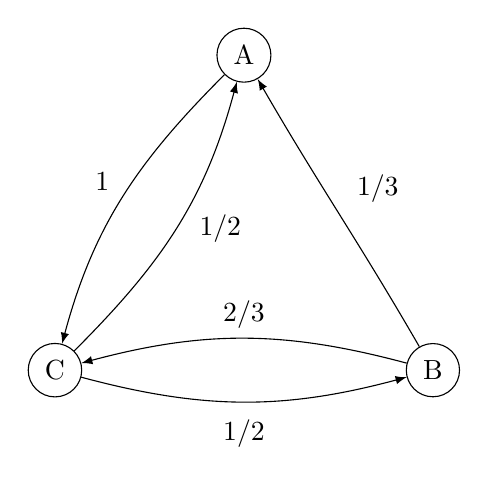
\begin{tikzpicture}
\node[draw,circle] (1)at(0,4){A};
\node[draw,circle] (2)at(-2.4,0){C};
\node[draw,circle] (3)at(2.4,0){B};
\draw[->,>=latex] (1) to[out=225,in=75] (2);
\draw[->,>=latex] (2) to[out=45,in=255] (1);
\draw[->,>=latex] (2) to[out=-15,in=195] (3);
\draw[->,>=latex] (3) to[out=120,in=-60] (1);
\draw[->,>=latex] (3) to[out=165,in=15] (2);
\node at(-1.8,2.4) {$1$};
\node at(-0.3,1.8) {$1/2$};
\node at(0,-0.8) {$1/2$};
\node at(0,0.7) {$2/3$};
\node at(1.7,2.3) {$1/3$};
\end{tikzpicture}
\]
La matrice de transition $Q$ associée à $(X_n)_{n\geq0}$ est définie par :
\[
Q=\begin{pmatrix}
0 & 0 & 1 \\
1/3 & 0 & 2/3  \\
1/2 & 1/2 & 0
\end{pmatrix}.
\]
\end{solution}
\part Notons, pour tout $n\in\N$, $\mu_n = (a_n , b_n , c_n )$ la loi de $X_n$ .
\begin{itemize}
\item[(i)] Pour tout $n\in\N$, calculer $\mu_{n+1}$ en fonction de $\mu_n$.
\item[(ii)] On suppose que Anna a le ballon au début du jeu. Pour chacun des joueurs, calculer la probabilité d’avoir le ballon après deux lancers.
\end{itemize}
\begin{solution}
\begin{itemize}
\item[(i)] Puisque $(X_n)_{n\in\N}$ est une chaîne de Markov homogène, pour tout $n\in\N$, on a:
\[
\mu_{n+1}=\mu_{n} Q.
\]
\item[(ii)] Calculer la probabilité d’avoir le ballon après deux lancers pour chacun des joueurs revient à calculer $\mu_2$ pour $\mu_0=(1,0,0)$. On a:
\[
\mu_1 = \mu_0 Q = (0,0,1).
\]
De même,
\[
\mu_2 = \mu_1 Q = (1/2,1/2,0).
\]
On en conclut qu'après deux lancers, Carole n'a presque jamais le ballon, alors qu'Anne et Bruno ont chacun le ballon avec probabilité $1/2$.
\end{itemize}
\end{solution}
\part Montrer que $(X_n)_{n\geq0}$ admet une unique probabilité invariante $\pi$ et la calculer.
\begin{solution}
Une probabilité invariante $\pi:=(\pi_A,\pi_B,\pi_C)$ satisfait le système suivant :
\[
\left\{ \begin{matrix*}[l] 
\pi_A = \frac{1}{3}\pi_B + \frac{1}{2}\pi_C \\[+10pt]
\pi_B = \frac{1}{2}\pi_C \\
\pi_C = \pi_A + \frac{1}{2}\pi_B \\
\pi_A +\pi_B + \pi_C =1
\end{matrix*} \right.
\]
La seule solution de ce système est $\pi=\left(\frac{4}{13},\frac{3}{13},\frac{6}{13}\right)$.
\end{solution}
\end{parts}
\question On considère la chaîne de Markov sur l'espace d'états $\left\lbrace 1,2\right\rbrace$  dont la matrice de transition est la suivante : \\
\begin{center}
 $ \begin{pmatrix}
1-p & p \\
q & 1-q
\end{pmatrix}$
\end{center}
où $p,q \in \left[0,1 \right]$ sont fixés.
\begin{parts}
\part Dessiner son graphe. Déterminer la ou les mesures stationnaires.
\begin{solution}
Le graphe de la chaîne de Markov est donné par :
\[
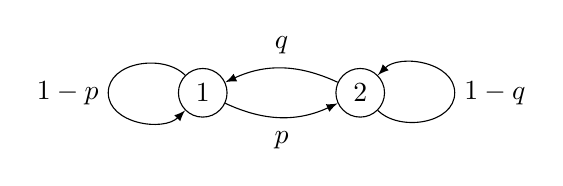
\begin{tikzpicture}
\node[draw,circle] (1)at(-1,0){1};
\node[draw,circle] (2)at(1,0){2};
\draw[-,>=latex] (1) to[out=135,in=90] (-2.2,0)node[left]{$1-p$};
\draw[->,>=latex] (-2.2,0)node{} to[out=-90,in=225] (1);
\draw[->,>=latex] (1) to[out=-25,in=205] (2);
\draw[-,>=latex] (2) to[out=-45,in=-90] (2.2,0)node[right]{$1-q$};
\draw[->,>=latex] (2.2,0)node{} to[out=90,in=45] (2);
\draw[->,>=latex] (2) to[out=155,in=25] (1);
\node at(0,0.6) {$q$};
\node at(0,-0.6) {$p$};
\end{tikzpicture}
\]
Une probabilité invariante $\pi=(\pi_1,\pi_2)$ satisfait le système suivant:
\[
\left\{ \begin{matrix*}[l] 
\pi_1 = (1-p)\pi_1 + q\pi_2 \\
\pi_2 = p\pi_1 + (1-q)\pi_2 \\
\pi_1 +\pi_2 =1
\end{matrix*} \right.
\]
Si $p=q=0$, la matrice de transition est l'identité et toute mesure de probabilité est une mesure de probabilité invariante.\\
Sinon, il y a  une unique mesure de probabilité invariante : 
\[
\pi=(q/(p+q),p/(p+q)).
\]
\end{solution}
\part On note $a_n = P(X_n = 1)$ et $b_n = \P(X_n = 2)$. Ecrire une relation de récurrence pour les couples $(a_n, b_n)$ et la résoudre.
\begin{solution}
On a, pour tout $n\in\N$ :
\[
(a_{n+1},b_{n+1})=(a_n,b_n) Q.
\]
De plus $b_n=\P(X_n = 2)=1-\P(X_n = 1)=1-a_n$. Cela signifie que pour tout $n\in\N$ :
\[
a_{n+1}=(1-p)a_n+q(1-a_n)=(1-p-q)a_n+q.
\]
Si $p=q=0$, on a $(a_n,b_n)=(a_0,b_0)$.\\
Sinon, on a une suite arithmético-géométrique et 
\[
a_n=\frac{q}{p+q}+(1-p-q)^n\left(a_0-\frac{q}{p+q}\right).
\]
De même,
\[
b_n=\frac{p}{p+q}+(1-p-q)^n\left(b_0-\frac{p}{p+q}\right).
\]
\end{solution}
\part Etudier alors le comportement asymptotique de $\P(X_n = 1)$.
\begin{solution}
On a trois cas de figures possible :
\begin{itemize}
\item si $p=q=0$, $\P(X_n = 1)=\P(X_0 = 1)$. En particulier la suite converge.
\item si $p=q=-1$, $\P(X_n = 1)= 1/2 + (-1)^n(\P(X_0 = 1)-1/2)$ donc la suite ne converge pas sauf si $\P(X_0 = 1)=1/2$ auquel cas la suite est stationnaire.
\item sinon, $\P(X_n = 1)$ converge exponentiellement vite vers $q/(p+q)$ qui correspond à la probabilité invariante.
\end{itemize}
\end{solution}
\end{parts}
\question \textbf{Dépenses énergétiques} \\
On dispose, dans une maison individuelle, de deux systèmes de chauffage, l'un de base, et l'autre d'appoint. On dira qu'on est dans l'état 1 si seul le chauffage de base fonctionne, et dans l'état 2 si les deux systèmes fonctionnent. \\
Si un jour on est dans l'état 1, on estime qu'on y reste le lendemain avec une probabilité $\dfrac{1}{2}$ ; en revanche, si on est dans l'état 2, le lendemain la maison est chaude, et l'on passe à l'état 1 avec une probabilité $\dfrac{3}{4}$. \\
Soit $X_n$ l'état du système au jour numéro $n$.
\begin{parts}
\part Expliquer pourquoi $(X_n)_{n \geq 0}$ peut être modélisé par une chaîne de Markov homogène. Quel est son espace d'états ? Déterminer sa matrice de transition $Q$ et son graphe.
\begin{solution}
On sait que la probabilité d'être dans un état un jour ne dépend que de l'état le jour précédent, on peut donc modéliser le problème par une chaîne de Markov. Les probabilités de transitions ne dépendant pas du jour, la chaîne de Markov est homogène. L'espace d'états comporte deux états : l'état 1 (chauffage de base) et l'état 2 (les deux systèmes). La matrice de transition $Q$ est donnée par :
\[
Q:=\left(
\begin{matrix}
1/2 & 1/2 \\
3/4 & 1/4
\end{matrix}
\right)
\]
et le graphe par :
\[
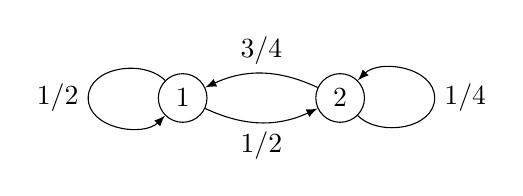
\begin{tikzpicture}
\node[draw,circle] (1)at(-1,0){1};
\node[draw,circle] (2)at(1,0){2};
\draw[-,>=latex] (1) to[out=135,in=90] (-2.2,0)node[left]{$1/2$};
\draw[->,>=latex] (-2.2,0)node{} to[out=-90,in=225] (1);
\draw[->,>=latex] (1) to[out=-25,in=205] (2);
\draw[-,>=latex] (2) to[out=-45,in=-90] (2.2,0)node[right]{$1/4$};
\draw[->,>=latex] (2.2,0)node{} to[out=90,in=45] (2);
\draw[->,>=latex] (2) to[out=155,in=25] (1);
\node at(0,0.6) {$3/4$};
\node at(0,-0.6) {$1/2$};
\end{tikzpicture}
\]
\end{solution}
\part On pose $p_n = \P(X_n = 1)$. Déterminer une relation de récurrence entre $p_n$ et $p_{n+1}$, puis exprimer $p_n$ en fonction de $p_0$. Que vaut $\lim _{n\longrightarrow \infty} p_n$ ?
\begin{solution}
On sait que :
\[
(p_{n+1}, 1-p_{n+1})=(p_n, 1-p_n) Q.
\] 
On a donc 
\[
p_{n+1}= \frac{1}{2} p_n + \frac{3}{4} (1-p_n)= -\frac{1}{4} p_n +\frac{3}{4}.
\]
On a une suite arithmético-géométrique donc
\[
p_n=\frac{3}{5} + \left(-\frac{1}{4}\right)^n\left(p_0-\frac{3}{5}\right).
\]
On en conclut que la suite $(p_n)_{n\in\N}$ converge vers $\frac{1}{3}$.
\end{solution}
\part Sachant qu'on est dans l'état 1 un dimanche, trouver la probabilité d'être dans le même état le dimanche suivant ?
\begin{solution}
On cherche à calculer $\P\left(X_{n+7}=1|X_n=1\right)$. La chaîne étant homogène, cela revient à calculer $\P(X_7=1|X_0=1)$. Si on utilise les notations de la question précédente, cela revient à calculer $p_7$ pour $p_0=1$. On trouve, d'après la question précédente :
\[
\P(X_7=1|X_0=1)=\frac{3}{5} + \frac{2}{5}\left(-\frac{1}{4}\right)^7.
\]
\end{solution}
\part Montrer que si un jour on se trouve dans l'état 1 avec une proba $\dfrac{3}{5}$, alors il en est de même tous les jours qui suivent.
\begin{solution}
On peut montrer ce résultat par récurrence. Soit $p_n$ la probabilité d'être dans l'état 1 le jour $n$. On sait que $p_0=\frac{3}{5}$. Pour tout $n\in\N$, si $p_n=\frac{3}{5}$ alors :
\[
\begin{aligned}
p_{n+1}=& p_n \P(X_{n+1}=1|X_n=1)+ (1-p_n) \P(X_{n+1}=1|X_n=2)\\
=& \frac{3}{5}\times  \frac{1}{2} + \frac{2}{5}\times  \frac{3}{4}\\
=& \frac{3}{5}.
\end{aligned}
\]
Par récurrence on en conclut que si un jour on est dans l'état $1$ avec probabilité $3/5$ alors tous les jours suivant on est également dans l'état $1$ avec probabilité $3/5$.
\end{solution}
\part Chaque journée dans l'état 1 coûte 1,5\euro, et dans l'état 2 coûte 2\euro. Chaque transition de l'état 1 à l'état 2 ou inversement coûte 0,5\euro. Calculer le coût moyen d'une journée dans la situation précédente.
\begin{solution}
Dans la situation précédente, toutes les journées sont dans l'état 1 avec probabilité $3/5$ et dans l'état $2$ avec probabilité $2/5$. Une journée dans cette situation coûte donc en moyenne :
\[
\begin{aligned}
&\P(X_n=1)\times  1,5 + \P(X_{n+1}=2 \text{ et } X_n=1) \times  0,5  \\
& \ \ \ \ \ \ \  +\P(X_n=2)\times  2 + \P(X_{n+1}=1 \text{ et } X_n=2) \times  0,5\\
=& \frac{3}{5}\times 1,5 + \frac{3}{5}\times \frac{1}{2} \times  0,5 + \frac{2}{5}\times 2 + \frac{2}{5}\times \frac{3}{4} \times  0,5
=2\euro.
\end{aligned}
\]
\end{solution}
\end{parts}
\question \textbf{Bruit qui court} \\
Un message pouvant prendre 2 formes (oui ou non) est transmis à travers $n$ intermédiaires. On suppose que chaque intermédiaire transmet le message de façon correcte avec une probabilité $p \in \left] 0, 1\right[ $ ou le déforme en son contraire avec une probabilité $1 - p$. Les intermédiaires sont
indépendants.
\begin{parts}
\part Modéliser cette situation par une chaîne de Markov à 2 états.
\begin{solution}
On peut modéliser la situation par la chaîne de Markov donnée par le graphe suivant : 
\[
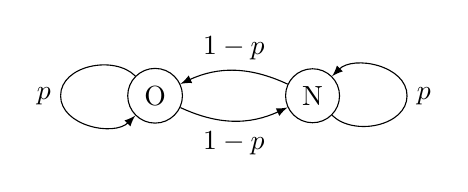
\begin{tikzpicture}
\node[draw,circle] (1)at(-1,0){O};
\node[draw,circle] (2)at(1,0){N};
\draw[-,>=latex] (1) to[out=135,in=90] (-2.2,0)node[left]{$p$};
\draw[->,>=latex] (-2.2,0)node{} to[out=-90,in=225] (1);
\draw[->,>=latex] (1) to[out=-25,in=205] (2);
\draw[-,>=latex] (2) to[out=-45,in=-90] (2.2,0)node[right]{$p$};
\draw[->,>=latex] (2.2,0)node{} to[out=90,in=45] (2);
\draw[->,>=latex] (2) to[out=155,in=25] (1);
\node at(0,0.6) {$1-p$};
\node at(0,-0.6) {$1-p$};
\end{tikzpicture}
\]
ce qui correspond à la matrice de transition 
\[
Q=\left(
\begin{matrix}
p & 1-p \\ 
1-p & p
\end{matrix}
\right)
\]
\end{solution}
\part Calculer la probabilité que l'information transmise par le n-ième intermédiaire soit conforme à l'information initiale. \\
\textit{Indication :} remarquer que (1, 1) et (1,-1) sont vecteurs propres de Q et diagonaliser Q.
\begin{solution}
On remarque que 
\[
\left( \begin{matrix}
p & 1-p \\ 
1-p & p
\end{matrix} \right)
\left( \begin{matrix}
1 \\ 
1
\end{matrix} \right)
= \left( \begin{matrix}
1 \\ 
1
\end{matrix} \right) \text{ et }
\left( \begin{matrix}
p & 1-p \\ 
1-p & p
\end{matrix} \right)
\left( \begin{matrix}
1 \\ 
-1
\end{matrix} \right)
= (2p-1)\left( \begin{matrix}
1 \\ 
-1
\end{matrix} \right).
\]
Soit $A$ la matrice définie par
\[
A= \left( \begin{matrix}
1 & 1 \\ 
1 & -1
\end{matrix} \right).
\]
L'inverse de $A$ est :
\[
A^{-1}= \frac{1}{2}\left( \begin{matrix}
1 & 1 \\ 
1 & -1
\end{matrix} \right).
\]
On a alors:
\[
A^{-1}QA= \left( \begin{matrix}
1 & 0 \\ 
0 & 2p-1
\end{matrix} \right).
\]
On en conclut donc que
\[
Q^n=A\left( \begin{matrix}
1 & 0 \\ 
0 & 2p-1
\end{matrix} \right)^nA^{-1}
=A\left( \begin{matrix}
1 & 0 \\ 
0 & (2p-1)^n
\end{matrix} \right)A^{-1}
=\frac{1}{2}\left( \begin{matrix}
1 +  (2p-1)^n & 1 - (2p-1)^n \\ 
1 -  (2p-1)^n & 1 +  (2p-1)^n
\end{matrix} \right)
\]
La probabilité que l'information transmise par le n-ième intermédiaire soit conforme à l'information initiale vaut donc $\frac{1+(2p-1)^n}{2}$.
\end{solution}
\part Que se passe-t-il lorsque $n \rightarrow + \infty$?
\begin{solution}
On a trois cas de figure possible :
\begin{itemize}
\item si $p=1$, l'information transmise est toujours conforme à l'information initiale, on n'a donc aucune perte d'information,
\item si $p=0$, l'information transmise est toujours conforme à l'information initiale lors des étapes paires, et est l'inverse de l'information initiale lors des étapes impaires,
\item sinon, la probabilité que l'information transmise à l'étape $n$ soit conforme à l'information initiale converge vers $\frac{1}{2}$.
\end{itemize}
\end{solution}
\end{parts}
\end{questions}
\end{document}
